In this LIDAR lab oration the National instruments myRIO was used in combination with National instruments LabWIEV. 
When using myRIO as an base for the LIDAR there is a coupel of design considerations to take in to count especially if the LIDAR have the need to be fast because then the latency and the transfer speed of the USB can be a limitation. 
In this report it was decided that we use a spitted architecture letting the myRIO do the measurements and controlling the motor while the personal computer was used to display the data that the myRIO captured.
\subsection{The myRIO software}\label{subsection:myRIO}
\begin{figure}[ht]
%  \includegraphics[scale=1.7]{birds.jpg}
    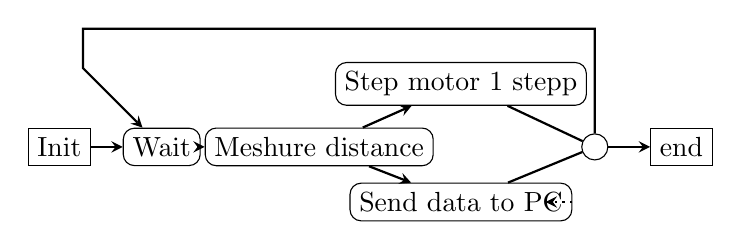
\begin{tikzpicture}
\tikzstyle{startstop} = [rectangle, rounded corners , minimum width=3mm, minimum height=1mm,text centered, draw=black]
\tikzstyle{round}=[circle, minimum width=0mm,draw=black]
\tikzstyle{first} = [rectangle, minimum width=1mm, draw=black]
\tikzstyle{empty}=[]

\usetikzlibrary{shapes.geometric, arrows}
\tikzstyle{arrow} = [thick,->,>=stealth]
\tikzstyle{dottarrow} = [thick, dotted,->,>=stealth]
\tikzstyle{noarrow}=[thick,-=,=stealth]

%nodes
\node (init) [first] {Init};
\node (wait) [startstop, right of =init, xshift=3mm] {Wait};
\node (mesh) [startstop, right of=wait, xshift=10mm] {Meshure distance};
\node (step) [startstop, right of=mesh, xshift=8mm ,yshift=8mm] {Step motor 1 stepp};
\node (send) [startstop, below of=step, yshift=-5mm]{Send data to PC};
\node (merge) [round, right of=mesh, yshift=0mm, xshift=25mm]{};
\node (end) [first, right of=merge, xshift=1mm] {end};
\node (topc) [empty, right of=send, xshift=2mm]{};

%arrows
\draw [arrow] (wait) -- (mesh);
\draw [arrow] (init) -- (wait);
\draw [arrow] (mesh) -- (step);
\draw [arrow] (mesh) -- (send);
\draw [noarrow] (send) -- (merge);
\draw [noarrow] (step) -- (merge);
\draw [dottarrow] (send) -- (topc);
\draw [arrow] (merge)  -- +(0,1.5)  -- (0.3,1.5) -- (0.3,1) -- (wait);
\draw [arrow] (merge) -- (end);
\end{tikzpicture}
  \caption{This figure describes the inner simplified working of the myRIO code.
  At initialize we initialize the unit. Then because how the myRIO is working we wait while the myRIO is measuring the sensor. The measure block only represents that we retrieve the value of the previously measured data. The data is put on the FIFO stack to b sent to the computer while myRIO takes an other step with the stepper motor. When that is done and the user haven't pressed stop to abort we loop back to wait and do the measurement again.}
  \label{fig:myRIO-loop}
\end{figure}
The myRIO part of the code uses an loop described in figure \ref{fig:myRIO-loop}.
\subsubsection{Step motor control}\label{subsubsection:Step-control}
Step motor control is achieved by using a implementation of a shift register explained in figure \ref{fig:shift-reg}. 
\begin{figure}[ht]
%  \includegraphics[scale=1.7]{birds.jpg}
    %\centering
%   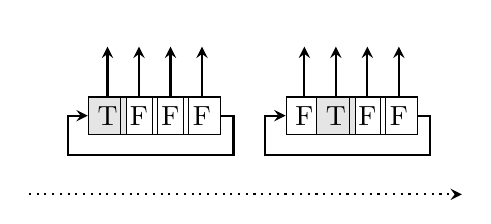
\begin{tikzpicture}
\tikzstyle{notused} = [rectangle, rounded corners , minimum width=3mm, minimum height=1mm,text centered, draw=black]
\tikzstyle{round}=[circle, minimum width=0mm,draw=black]
\tikzstyle{square} = [rectangle, minimum width=1mm, draw=black]
\tikzstyle{qraysquare} = [
rectangle, minimum width=1mm, draw=black, fill=gray!20]
\tikzstyle{empty}=[]

\usetikzlibrary{shapes.geometric, arrows}
\tikzstyle{arrow} = [thick,->,>=stealth]
\tikzstyle{dottarrow} = [thick, dotted,->,>=stealth]
\tikzstyle{noarrow}=[thick,-=,=stealth]

%node
\node (DA) [qraysquare] {T};
\node (DB) [square, right of =DA, xshift=-6mm] {F};
\node (DC) [square, right of =DB, xshift=-6mm] {F};
\node (DD) [square, right of =DC, xshift=-6mm] {F};

\node (DE) [square, right of =DD, xshift=3mm] {F};
\node (DF) [qraysquare, right of =DE, xshift=-6mm] {T};
\node (DG) [square, right of =DF, xshift=-6mm] {F};
\node (DH) [square, right of =DG, xshift=-6mm] {F};

%Epmty target nodes
\node (DAT) [empty, yshift=10mm]{};
\node (DBT) [empty, right of=DAT, xshift=-6mm]{};
\node (DCT) [empty, right of=DBT, xshift=-6mm]{};
\node (DDT) [empty, right of=DCT, xshift=-6mm]{};

\node (DET) [empty, right of=DDT, xshift=3mm]{};
\node (DFT) [empty, right of=DET, xshift=-6mm]{};
\node (DGT) [empty, right of=DFT, xshift=-6mm]{};
\node (DHT) [empty, right of=DGT, xshift=-6mm]{};

%lines to target node
\draw [arrow] (DA) -- (DAT);
\draw [arrow] (DB) -- (DBT);
\draw [arrow] (DC) -- (DCT);
\draw [arrow] (DD) -- (DDT);
\draw [arrow] (DD)  -- +(0.4,0) -- +(0.4,-0.5) -- (-0.5,-0.5) -+(-0.5,0.0) -- +(DA);

\draw [arrow] (DE) -- (DET);
\draw [arrow] (DF) -- (DFT);
\draw [arrow] (DG) -- (DGT);
\draw [arrow] (DH) -- (DHT);
\draw [arrow] (DH)  -- +(0.4,0) -- +(0.4,-0.5) -- (2.0,-0.5) -+(2.0,0.0) -- +(DE);

\draw [dottarrow] (-1.0cm,-1.0cm) -- (4.5cm,-1cm);

%node (D1) [square right of=Dfirst, xshift=8mm] {F};
%\node (D2) [square right of=D1, xshift=8mm] {F};
\end{tikzpicture}
  \caption{The shift register is working by step wise shifting the true state on step to the right. When the true state reaches the right most cell it will on the next step be shifted to the beginning of the register.}
  \label{fig:shift-reg}
\end{figure}